\documentclass[12pt]{extreport}

\usepackage[english]{babel}
\usepackage[utf8x]{inputenc}
\usepackage[T1]{fontenc}
\usepackage{listings}
\usepackage{hyperref}
\hypersetup{colorlinks=false}
\usepackage{lscape}
\usepackage{subfigure}
\usepackage{amsmath}
\usepackage{graphicx}
\usepackage[colorinlistoftodos]{todonotes}
\usepackage{}
\usepackage{mips}
\usepackage{titlesec}

\titleformat{\chapter}
  {\Large\bfseries} % format
  {}                % label
  {0pt}             % sep
  {\huge}

% the following is needed for syntax highlighting
\usepackage{color}

\definecolor{dkgreen}{rgb}{0,0.6,0}
\definecolor{gray}{rgb}{0.5,0.5,0.5}
\definecolor{mauve}{rgb}{0.58,0,0.82}


\lstset{ %
  language=[mips]Assembler,       % the language of the code
  basicstyle=\footnotesize,       % the size of the fonts that are used for the code
  numbers=left,                   % where to put the line-numbers
  numberstyle=\tiny\color{gray},  % the style that is used for the line-numbers
  stepnumber=1,                   % the step between two line-numbers. If it's 1, each line 
                                  % will be numbered
  numbersep=5pt,                  % how far the line-numbers are from the code
  backgroundcolor=\color{white},  % choose the background color. You must add \usepackage{color}
  showspaces=false,               % show spaces adding particular underscores
  showstringspaces=false,         % underline spaces within strings
  showtabs=false,                 % show tabs within strings adding particular underscores
  frame=single,                   % adds a frame around the code
  rulecolor=\color{black},        % if not set, the frame-color may be changed on line-breaks within not-black text (e.g. commens (green here))
  tabsize=4,                      % sets default tabsize to 2 spaces
  captionpos=b,                   % sets the caption-position to bottom
  breaklines=true,                % sets automatic line breaking
  breakatwhitespace=false,        % sets if automatic breaks should only happen at whitespace
  title=\lstname,                 % show the filename of files included with \lstinputlisting;
                                  % also try caption instead of title
  keywordstyle=\color{blue},          % keyword style
  commentstyle=\color{dkgreen},       % comment style
  stringstyle=\color{mauve},         % string literal style
  escapeinside={\%*}{*)},            % if you want to add a comment within your code
  morekeywords={*,...}               % if you want to add more keywords to the set
}

%% Sets page size and margins
\usepackage[a4paper,top=3cm,bottom=2cm,left=3cm,right=3cm,marginparwidth=1.75cm]{geometry}

\title{An Implementation Study of Register Renaming Logic}
% Update supervisor and other title stuff in title/title.tex

\begin{document}
\begin{titlepage}

\newcommand{\HRule}{\rule{\linewidth}{0.5mm}} % Defines a new command for the horizontal lines, change thickness here

%----------------------------------------------------------------------------------------
%	LOGO SECTION
%----------------------------------------------------------------------------------------


\includegraphics[width=4cm]{title/logo.jpg}\\[1cm] % Include a department/university logo - this will require the graphicx package
 
%----------------------------------------------------------------------------------------

\center % Center everything on the page

%----------------------------------------------------------------------------------------
%	HEADING SECTIONS
%----------------------------------------------------------------------------------------
\quad\\[1.5cm]
%\textsc{\LARGE MSc Thesis}\\[1.5cm] % Name of your university/college
\textsc{\Large Indian Institute of Technology Roorkee}\\[0.5cm] % Major heading such as course name
\textsc{\large Computer Architecture and Microprocessors}\\[0.5cm] % Minor heading such as course title

%----------------------------------------------------------------------------------------
%	TITLE SECTION
%----------------------------------------------------------------------------------------
\makeatletter
\HRule \\[0.4cm]
{ \huge \bfseries \@title}\\[0.4cm] % Title of your document
\HRule \\[1.5cm]
 
%----------------------------------------------------------------------------------------
%	AUTHOR SECTION
%----------------------------------------------------------------------------------------

\begin{minipage}{0.4\textwidth}
\begin{flushleft} \large
\emph{Author:}\\
Anupam Singh \\*
Katkar Prathamesh Shivaji \\*
Utkarsh \\*
Sanskar Agarwal \\*
Harshit Goenka \\*
Shivam Yadav \\*
Jitendra Patel
\end{flushleft}
\end{minipage}
~
\begin{minipage}{0.4\textwidth}
\begin{flushright} \large
\emph{Supervisor:} \\
Sateesh Kumar Peddoju 
% Uncomment the following lines if there's a co-supervisor
%\\[1.2em] % Supervisor's Name
%\emph{Co-Supervisor:} \\
%Dr. Adam Smith % second marker's name
\end{flushright}
\end{minipage}\\[3cm]
\makeatother


%----------------------------------------------------------------------------------------
%	DATE SECTION
%----------------------------------------------------------------------------------------

{\large A report submitted for our project on}\\[0.5cm]
{\large \emph{Register Renaming Logic}}\\[0.5cm]
{\large \today}\\[2cm] % Date, change the \today to a set date if you want to be precise

\vfill % Fill the rest of the page with whitespace

\end{titlepage}

\begin{abstract}
Most modern computer applications require that the computer system meets minimum requirements in order to run. One of those requirements is processor’s performance. Computer architects are trying to improve a processor's performance in every way possible. \\
One of the ways of improving processor's performance is register renaming. A register is a small unit of fast storage quickly accessible to a computer's CPU. Every logical register has a set of physical registers associated with it. While a programmer in assembly language refers, for instance to a logical register \textbf{\$r0}, the processor transposes this name to one specific physical register. The physical registers are opaque and cannot be referenced directly but only via the canonical names. This property of CPU registers can be exploited to improve CPU performance. If in an assembly language, multiple instructions refer to the same registers (i.e. having same canonical names), but these instructions are independent of each other, we can simply change the canonical name of some of these registers. This will make these instructions eligible for parallel execution, thus reducing the number of CPU cycles per instruction. This helps to reveal more instruction level parallelism in an instruction stream. \\
Register renaming helps to remove false data dependencies. This project will help us understand how this elegant technique is implemented in modern processors and how it affects the CPU performance. This project will cover some register renaming algorithms (implementation and analysis).

\end{abstract}
\tableofcontents
\chapter{Why we choose this topic?}

Pipeline hazards prevent next instruction from executing during designated clock cycle.There are 3 classes of pipeline hazards one of them is data hazards which occur when given instruction depends on data from an instruction ahead of it in pipeline.To eliminate data hazards one of the ways is register renaming.	

Register renaming is an elegant technique which helps to remove data hazards: Write after Read(False Dependency) and Write after Write(False Dependency).The principle of register renaming is straightforward. If the processor encounters an instruction that addresses a destination register, it temporarily writes the instruction’s result into a dynamically allocated rename buffer rather than into the specified destination register.Renaming increases the average number of instructions that are available for parallel execution per cycle.

This technique is interesting because virtually all recent superscalars rename registers to boost performance and system performance.Besides this data hazards and pipelining are in our \textbf{CSN 221} course structure so we find it amusing to gain in depth knowledge about eliminating data hazards.

\chapter{Gantt Chart}

\section{Tasks}
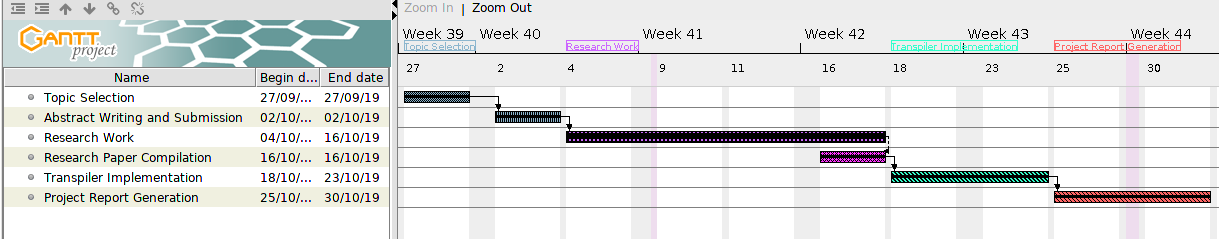
\includegraphics[width=15cm]{gantt/tasks.png}\\[1cm]

\section{Resources}

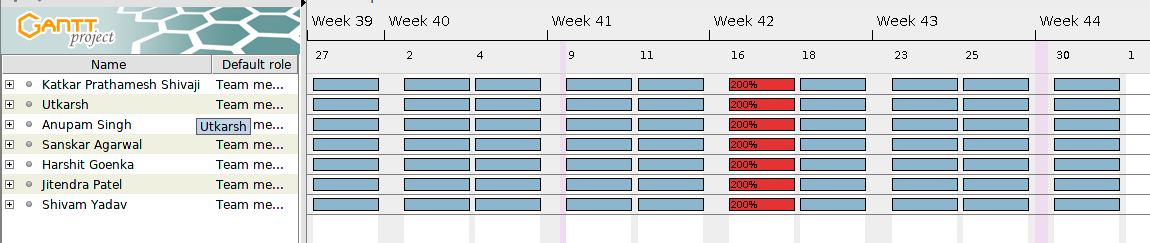
\includegraphics[width=15cm]{gantt/resources.png}\\[1cm]

\section{PERT Chart}

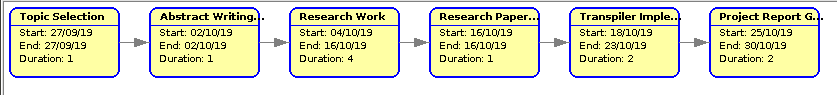
\includegraphics[width=15cm]{gantt/pert.png}\\[1cm]
\chapter{Background}
\section{Hazards}
Instructions in a pipelined processor are performed in several stages, so that at any given time several instructions are being processed in the various stages of the pipeline which helps to increase clock frequency.  A hazard occurs when two or more of these simultaneous instructions conflict in the pipeline.


Data hazards occur when instructions that exhibit data dependence modify data in different stages of a pipeline. There are three situations in which a data hazard can occur:
\begin{itemize}
  \item Read after Write (True data dependency)
  \item Write after Read (False data dependency)
  \item Write after Write (False data dependency)
\end{itemize}
\subsection{Read after write (RAW)}
A read after write (RAW) data hazard refers to a situation where an instruction refers to a result that has not yet been calculated or retrieved. This can occur because even though an instruction is executed after a prior instruction, the prior instruction has been processed only partly through the pipeline.
\\*
For example:
\begin{lstlisting}
add $t2,$t1,$t3
add $t4,$t2,$t3
\end{lstlisting}
The first instruction is calculating a value to be saved in register \$t2, and the second is going to use this value to compute a result for register \$t4. However, in the pipeline, when operands are fetched for the 2nd instructions, the results from the first will not yet have been saved, and hence a data dependency occurs.

A data dependency occurs with instruction i2, as it is dependent on the completion of instruction i1. This type is dependency is unaffected by register renaming.

\subsection{Write after read (WAR)}
A write after read (WAR) data hazard represents a problem with concurrent execution.  \\*
For Example:
\begin{lstlisting}
add $t4,$t1,$t5
add $t5,$t1,$t2
\end{lstlisting}

In pipelining situation there is a chance that i2 may finish before i1, it must be ensured that the result of register \$t5 is not stored before i1 has had a chance to fetch the operands. It can be easily solved by register renaming.

\subsection{Write after write (WAW)}
(i2 tries to write an operand before it is written by i1) A write after write (WAW) data hazard may occur in a concurrent execution environment. \\*
For example:
\begin{lstlisting}
add $t2,$t4,$t7 
add $t2,$t1,$t3
\end{lstlisting}

The write back of i2 must be delayed until i1 finishes executing. It can be easily solved by register renaming.

\section{Role of Register Renaming}
Write after Read and Write after Write are two false dependencies which can be resolved by register renaming. Instead of delaying the write operation until all read operations are completed, two copies of the location can be maintained, the old value and the new value. Read operation that happens before the write operation of the new value can be provided with the old value while other read operations that follow the write operations are provided with the new value. The false dependency is broken and additional opportunities for out-of-order execution are created. When all reads that need the old value have been satisfied, it can be discarded. This is the essential concept behind register renaming.
\chapter{Register Renaming Technique}
Register renaming is a technique used to allow multiple execution paths without conflicts between different execution units trying to use the same registers.Instead of just one set of registers being used,multiple sets are put into the processor.This allows different execution units to work simultaneously without unnecessary pipeline stalls. For many computations, a CPU uses the data stored in its registers.Processors with large no of registers can use them to hold many program variables,which reduces the number of cache and external memory accesses. Register renaming technique used in all current processors based on the x86 instruction set, can eliminate this false dependency by dynamically substituting different physical registers when dealing with closely-grouped independent operations. Internally, renaming requires more physical registers than the logical registers that are visible to the outside world.
Register renaming distinguishes two kinds of registers: logical and physical registers.Logical registers are those used by the compiler,whereas physical registers are those actually implemented in the machine. Typically, the number of physical registers is quite larger than the number of logical registers. When an instruction that produces a result is decoded, the renaming logic allocates a free physical register. The logical destination register is said to be mapped to that physical register. Subsequent data dependent instructions rename their source registers to access this physical register.



\chapter{Theory}
\section{Reorder Buffer}
Renaming based on a reorder buffer uses a physical register file that is the same size as the architectural register file, together with a set of registers arranged as a queue data structure, called the reorder buffer

As instruction execution proceeds, the assigned entry will ultimately be filled in by a value, representing the result of the instruction. When entries reach the head of the reorder buffer, provided they've been filled in with their actual intended result, they are removed, and each value is written to its intended architectural register. If the value is not yet available, then we must wait until it is.

Because instructions take variable times to execute, and because they may be executed out of program order, we may well find that the reorder buffer entry at the head of the queue is still waiting to be filled, while later entries are ready. In this case, all entries behind the unfilled slots must stay in the reorder buffer until the head instruction completes.

For example, consider the case of 6 instructions I1 – I6. Suppose at a given clock cycle that I1 and I2 both finish, and that at earlier clock cycles I4 to I6 also finished, but I3 is yet to complete. We can move the results for I1 and I2 out of the reorder buffer into their respective architectural registers. However, I4 to I6 must wait until I3 has completed.

\section{Tomasulo Algorithm}
Tomasulo’s algorithm is a computer architecture hardware algorithm for dynamic scheduling of instructions that allows out of order execution and enables more efficient use of multiple execution units. Every register is augmented by a busy bit. If the bit is off, the register holds the value needed by any instruction that references it. If the bit is set, the register holds the tag of the instruction that will produce the need value. When an instruction enters the decode stage, it is assigned a tag. It reads each source register, obtaining an input value or a tag, depending on the busy bit. The instruction writes its tag into its output register and sets that register’s busy bit. The instruction and its input values/tags are buffered in one of several reservation stations, depending on which functional unit it will execute in. At each cycle, a functional unit scans the instructions stored in its reservation station. An instruction may be ready, i.e., have both input values available, or waiting, i.e., one or more of its inputs is a tag, and the instruction cannot execute until some other instruction produces that input. The functional unit will select a ready instruction and start executing it. When an instruction completes, its result and tag are broadcast to all waiting instructions. Each waiting instruction compares this tag against the tags it is waiting on. If the tags match, the instruction overwrites the tag with the result. This may change the instructions status from waiting to ready. The result is also sent to the register file. If the tag in the output register is the same as that of the instruction, the value is written to the register file.

Following concepts are important for implementing tomasulo’s algorithm:
\begin{itemize}
  \item Reservation station(RS)
  \item Common data bus(CDB)
  \item Register Renaming
\end{itemize}

\begin{enumerate}
  \item Reservation Status: it’s the buffer to store order of instruction
  \item Common Data Bus: The CDB connects reservation stations directly to functional units. According to Tomasulo it "preserves precedence while encouraging concurrency".
  \item Register Renaming: All general-purpose and reservation station registers hold either a real value or a placeholder value. If a real value is unavailable to a destination register during the issue stage, a placeholder value is initially used. The placeholder value is a tag indicating which reservation station will produce the real value. When the unit finishes and broadcasts the result on the CDB, the placeholder will be replaced with the real value.
\end{enumerate}
\chapter{Implementation}

We have implemented a simplified version of register renaming model explained in the paper.
As explained in the paper, the renaming of the register is done in the fetch cycle instead of decode cycle. This helps to eliminate false dependencies before complex pipeline phases. The program we have implemented is a simple asm transpiler which translates the MIPS assembly code to MIPS assembly code replacing the corresponding register. Since the asm file is statically transpiled, therefore control dependencies are impossible to demonstrate.
Since the architected registers are mapped onto some subset of the available physical registers, therefore we are using a subset of temporal MIPS register for architecture register.
MIPS architecture contains 10 temporal registers (named \$t0 to \$t9)
Now imagine a machine containing 10 physical temporal  register ($t0 to $t9) and 6 architecture register ($t0 to $t5). So sample assembly code can only use those 6 architecture register for demonstration purpose. The transpiler will convert the assembly code and remove false dependencies by mapping those architecture register ($t0 to $t5) to ($t0 to $t9). Please note that actual renaming is register is not happening at hardware level, we are only renaming it in the source code for demonstration purpose. \\* \\*
For example: \\* \\*
\textbf{Input MIPS code (input.asm)}

\begin{lstlisting}
.data
.text
main:
add $t0, $t1, $t2
add $t2, $t0, $t0
add $t0, $t0, $t0
\end{lstlisting}

\textbf{Transpiler commands}

\begin{lstlisting}[language=bash]
  $ ./register-renaming input.asm output.asm
  input file:input.asm
  output file:output.asm
\end{lstlisting}

\textbf{Output MIPS code (output.asm)}

\begin{lstlisting}
.data
.text
main:
add $t2, $t0, $t1
add $t3, $t2, $t2
add $t4, $t2, $t2
\end{lstlisting}
\chapter{References}

\section{Register Renaming and Dynamic Speculation: an Alternative Approach}
by Mayan Moudgill \& Keshav Pingali Stamatis Vassiliadis Department of Computer Science, School of Electrical Engineering, IBM Corporation, Cornell University, Cornell University, Enterprise Systems, Ithaca, NY 14853. Ithaca, NY 14853. Poughkeepsie, NY 12602. September 15, 1993\\
\url{http://citeseerx.ist.psu.edu/viewdoc/download?doi=10.1.1.59.4027&rep=rep1&type=pdf}

In this paper, they implemented register renaming, dynamic speculation and precise interrupts. Renaming of registers is performed during the instruction fetch stage instead of the decode stage, and the mechanism is designed to operate in parallel with the tag match logic used by most cache designs. By folding renaming into the instruction fetch stage, instead of implementing it in the instruction decode stage as competing approaches do, they remove complexity from the already-complex decode stage. 

\section{An Efficient Algorithm for Exploiting Multiple Arithmetic Units}
R. M Tomasulo\\
\url{https://pdfs.semanticscholar.org/8299/94a1340e5ecdb7fb24dad2332ccf8de0bb8b.pdf}

\section{The Design Space of Register Renaming Techniques}
D.Sima\\
\url{https://ieeexplore.ieee.org/stamp/stamp.jsp?tp=&arnumber=877952&tag=1}

\end{document}